% !TEX root =  ../mainPPDP.tex
%!TEX spellcheck = en_GB


In this section, we introduce the notion of complementability and effective complementability for global types, 
then we present some notable subclasses that can be proved to be effectively complementable, e.g., global types 
commutation-closed global types, $\synchmodel$-realisable global-types, and global types
with sender-driven choice. 
We start with the definition of complementable global type:

\begin{definition}[Complement of a  Global Type]
    A global type $\comp{\gt}$ is a complement of $\gt$ 
    if $\existentialmsclanguageof{\gt}=
     \mscsetofmodel{\synchmodel}
    \setminus
    \existentialmsclanguageof{\comp{\gt}}$.
    We say that $\gt$ is {\em complementable} if it admits at least one complement.
\end{definition}

As exemplified below, not all global types are complementable. 
\begin{figure*}[ht]
    %\cinzia{move to appendix}
    \begin{tikzpicture}

    \node[state, initial, initial text={}] (0) at (0,0) {$q_0$};
    \node[state, accepting, color=blue] (1) at (2,4) {$q_1$};
    \node[state, accepting, color=teal] (2) at (2,-2) {$q_2$};
    \node[state, accepting, color=brown] (3) at (2,0) {$q_3$};
    \node[state, accepting, color=red] (4) at (4,2) {$q_4$};
    \node[state, accepting, color=red] (5) at (5,1) {$q_5$};
    \node[state, accepting, color=blue] (6) at (8,4) {$q_6$};
    \node[state] (7) at (6,4) {$q_7$};
    \node[state, accepting, color=blue] (8) at (10,4) {$q_8$};
    \node[state] (9) at (8,2) {$q_9$};
    \node[state, accepting, color=red] (10) at (10,2) {$q_{10}$};
    \node[state] (11) at (8,0) {$q_{11}$};
    \node[state, accepting, color=brown] (12) at (10,0) {$q_{12}$};
    \node[state] (13) at (6,-2) {$q_{13}$};
    \node[state, accepting, color=teal] (14) at (8,-2) {$q_{14}$};
    \node[state, accepting, color=teal] (15) at (10,-2) {$q_{15}$};

    \draw[->] (0) edge node [sloped,above] {$m_1$} (1);
    \draw[->] (0) edge node [sloped,below]{$m_2$} (2);
    \draw[->] (0) edge node [above] {$m_3$} (3);
    \draw[->, loop above] (1) edge node {$m_1$} (1);
    \draw[->, loop below] (2) edge node {$m_2$} (2);
    \draw[->, loop below] (3) edge node {$m_3$} (3);
    \draw[->] (1) edge node [left] {$m_3$} (3);
    \draw[->] (1) edge node [sloped, above] {$m_2$} (4);
    \draw[->] (4) edge node [sloped, above] {$m_2$} (5);
    \draw[->, loop right] (5) edge node [right] {$m_2$} (5);
    \draw[->] (4) edge node [below] {$m_3$} (9);
    \draw[->, bend right=20] (4) edge node [sloped, above] {$m_1$} (6);
    \draw[->, bend left] (6) edge node [sloped, below] {$m_2$} (7);
    \draw[->, bend left] (7) edge node [sloped, above] {$m_1$} (6);
    \draw[->] (6) edge node [above] {$m_3$} (8);
    \draw[->, loop right] (8) edge node [right] {$m_3$} (8);
    \draw[->, bend left] (9) edge node [above] {$m_2$} (10);
    \draw[->, bend left] (10) edge node [above] {$m_3$} (9);
    \draw[->, loop right] (10) edge node [right] {$m_2$} (10);
    \draw[->] (3) edge node [above] {$m_2$} (11);
    \draw[->, bend left] (11) edge node [above] {$m_3$} (12);
    \draw[->, bend left] (12) edge node [below] {$m_2$} (11);
    \draw[->] (2) edge node [above] {$m_1$} (13);
    \draw[->, bend left] (13) edge node [above] {$m_2$} (14);
    \draw[->, bend left] (14) edge node [below] {$m_1$} (13);
    \draw[->] (14) edge node [above] {$m_3$} (15);
    \draw[->, loop right] (15) edge node [right] {$m_3$} (15);

    % on ajoute des accolades
    \draw [decorate,decoration={brace,amplitude=5pt}, color=blue] (12,4.5) -- node [midway, right=1em] {$k_1>k_2$} (12,3.5) ;
    \draw [decorate,decoration={brace,amplitude=5pt}, color=red] (12,2.5) -- node [midway, right=1em] {$k_2>k_3$} (12,0.7) ;
    \draw [decorate,decoration={brace,amplitude=5pt}, color=brown] (12,0.6) -- node [midway, right=1em] {$k_3>k_2$} (12,-.6) ;
    \draw [decorate,decoration={brace,amplitude=5pt}, color=teal] (12,-1.5) -- node [midway, right=1em] {$k_2>k_1$} (12,-2.5) ;


\end{tikzpicture}
    \caption{A non-complementable global type
    \label{fig:non-complementable-gt-1}}
\end{figure*} 

\begin{figure}
    %\cinzia{move to appendix}
    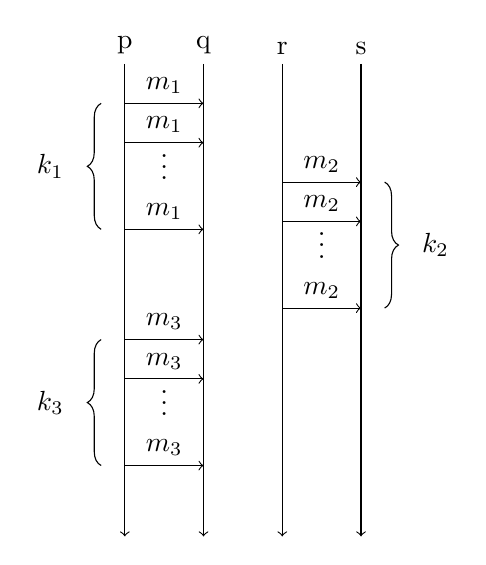
\begin{tikzpicture}
    \draw[->] (0,0) node [above] {p} -- (0,-6);
    \draw[->] (1,0) node [above] {q} -- (1,-6);
    \draw[->] (2,0) node [above] {r} -- (2,-6);
    \draw[->] (3,0) node [above] {s} -- (3,-6);

    \draw[->] (0,-.5) -- node [above] {$m_1$} (1,-.5);
    \draw[->] (0,-1) -- node [above] {$m_1$} (1,-1);
    \node at (.5,-1.2) {$\vdots$};
    \draw[->] (0,-2.1) -- node [above] {$m_1$} (1,-2.1);

    \draw[->] (2,-1.5) -- node [above] {$m_2$} (3,-1.5);
    \draw[->] (2,-2) -- node [above] {$m_2$} (3,-2);
    \node at (2.5,-2.2) {$\vdots$};
    \draw[->] (2,-3.1) -- node [above] {$m_2$} (3,-3.1);

    \draw[->] (0,-3.5) -- node [above] {$m_3$} (1,-3.5);
    \draw[->] (0,-4) -- node [above] {$m_3$} (1,-4);
    \node at (.5,-4.2) {$\vdots$};
    \draw[->] (0,-5.1) -- node [above] {$m_3$} (1,-5.1);

    % on ajoute des accolades
    \draw [decorate,decoration={brace,amplitude=5pt,mirror}] (-.3,-.5) -- node [midway, left=1em] {$k_1$} (-.3,-2.1) ;
    \draw [decorate,decoration={brace,amplitude=5pt,mirror}] (-.3,-3.5) -- node [midway, left=1em] {$k_3$} (-.3,-5.1) ;
    \draw [decorate,decoration={brace,amplitude=5pt}] (3.3,-1.5) -- node [midway, right=1em] {$k_2$} (3.3,-3.1) ;

\end{tikzpicture}

    \caption{The shape of the MSCs in $\msclanguageofcc{\gt_0}{}$ for the global type $\gt_0$.
    \label{fig:msc-regular}}
\end{figure} 

\begin{example}\label{ex:non-complementable-gt}
    Let $\Procs=\{p,q,r,s\}$, $\Messages=\{m_1,m_2,m_3\}$, and 
    $\Arrows=\{\gtlabel{p}{q}{m_1},\gtlabel{r}{s}{m_2},\gtlabel{p}{q}{m_3}\}$.
    First, consider a simple regular global type $\gt_0$ which MSCs linearisations 
    are of the form 
    $\{m_1^{k_1}m_2^{k_2}m_3^{k_3}\}$ (depicted in Fig.~\ref{fig:msc-regular}). 
    Note that $\gt_0$ is communitation-closed and
    $\existentialmsclanguageof{\gt_0}=\universalmsclanguageof{\gt_0}$.

    Second, consider the global type $\gt$ depicted in 
    Fig.~\ref{fig:non-complementable-gt-1}. 
    The linearisations of MSCs in $\existentialmsclanguageof{\gt}$ are 
    also of the form $\{m_1^{k_1}m_2^{k_2}m_3^{k_3}\}$ but 
    specifically with either $k_1\neq k_2$ or $k_2\neq k_3$.
    For instance, the upper branch of $\gt$ ensures that there is always at 
    least one $m_1$ more than $m_2$ in blue accepting states ($q_1$, $q_6$, $q_8$). 
    Similarly, the other branches ensure the other inequalities. 

    By contradiction suppose that  $\gt$ is complementable and  $\comp{\gt}$ is  its complement.
   Then $\gt''=\comp{\gt}\cap\gt_0$ exists and 
    since global type languages are closed under intersection with regular global types,
    $\gt''$ would still be a global type (in the form of a finite-state deterministic automaton).
    $\existentialmsclanguageof{\gt''}=\msclanguageofcc{\gt_0}{}\cap\existentialmsclanguageof{\gt'}$ 
    is the language of MSCs of the form %$\{m_1^{k_1}m_2^{k_2}m_3^{k_3}\}$ 
    %with $k_1=k_2=k_3$, i.e., all the MSCs of the form 
    $\{m_1^km_2^km_3^k\}$,  
    which no deterministic finite-state automaton, and therefore no global type, can recognise. 
    Thus, reaching a contradiction, hence $\gt''$, and $\comp{\gt}$ cannot exist, and $\gt$ is non-complementable.
\end{example}

\subsection{Effectively Complementable Global Types}

We say that complementation is effective for a class $\mathcal C$ of global types if 
there is a total, computable function $\gt \mapsto \comp{\gt}$ 
that takes as input a global type $\gt$ in $\mathcal C$ and computes its complement $\comp{\gt}$.

% \etienne{TODO changer les statements avec effective complementable.  
% Suggestions:
% - complementation is effective for a class of global types if 
% there is a procedure to effectively compute the complement of a given global type 
% in this class.
% - a class of global types is effectively complementable if there is a procedure to effectively compute the complement of a given global type in this class.
% }

\begin{proposition}\label{prop:commutation-closed-implies-complementable}
    Complementation is effective for the class of commutation-closed global types.
\end{proposition}

\begin{proof}
Let $\gt$ be a commutation-closed global type, and $Q,\delta$
be its  set of states and transition function. 
 $\comp{\gt}$ is the global type obtained by first completing 
$\gt$ (adding a sink state, so that the transition function $\delta:Q\times\Arrows\to Q$ is total),
and then swapping accepting and non-accepting states. 
Now, observe that 
$\existentialmsclanguageof{\comp{\gt}}=
\mscsetofmodel{\synchmodel}
\setminus \universalmsclanguageof{\gt}$. But, since $\gt$ is commutation closed:  
$\universalmsclanguageof{\gt}=\existentialmsclanguageof{\gt}$, concluding that 
$\comp{\gt}$ is a complement of $\gt$.
\end{proof}

As observed before, all global types with less than three participants are commutation closed, 
hence from Proposition~\ref{prop:commutation-closed-implies-complementable}
we have the following immediate result.

\begin{corollary}\label{coro:3-participants-complementable}
    Complementation is effective for the class of global types with $\cardinalof{\Procs}\leq 3$ participants.
\end{corollary}

More generally, we can show that all global types that are realisable in $\synchmodel$ 
are commutation-closed, and thus complementable.

\begin{theorem}\label{thm:realisable-complementable}
    Complementation is effective for the class of global types that are deadlock-free 
    realisable in $\synchmodel$.
\end{theorem}

\begin{proof}
    Let $\gt$ be a global type that is  deadlock-free realisable in $\synchmodel$.
    By condition~1 of Definition~\ref{def:realisability}, 
    $\executionsof{\projectionof{\gt}}{\synchmodel} = \executionsof{\gt}{\synchmodel}$.
    If two sets of executions are equal, the corresponding sets of their MSCs are also equal, 
    and thus $$\msclanguageof{\projectionof{\gt}}{\synchmodel}=\msclanguageof{\gt}{\synchmodel}.$$
    By construction, the synchronous product $\productof{\projectionof{\gt}}$
    is a global type whose runs are exactly the synchronous executions of the projected system, so 
    $$\msclanguageofcc{\productof{\projectionof{\gt}}}=\msclanguageof{\projectionof{\gt}}{\synchmodel}=\msclanguageof{\gt}{\synchmodel}.$$

    By Proposition~\ref{prop:product-is-commutation-closed}, $\productof{\projectionof{\gt}}$ is commutation-closed. 
    Thus, $\gt$ is also commutation-closed since they have the same MSCs language.
    Finally, by Proposition~\ref{prop:commutation-closed-implies-complementable},
    $\gt$ is complementable, and its proof  
    provides an effective algorithm for  complementation.
\end{proof}
    
\subsection{Sender-driven choice}

Stutz et al.  proved that $\ppmodel$-implementability (a notion close to realisability) 
is decidable for global types that satisfy sender-driven choice~\cite{DBLP:conf/cav/LiSWZ23}. We show that this can be seen as a consequence of the fact that global types with sender-driven choice are effectively complementable. We start by  recalling the definition of sender-driven choice.

\begin{definition}[Sender-driven choice]
    A global type $\gt$ has sender-driven choice
    if for all state $s$ of $\gt$, if $\gtlabel{p}{q}{m}$ and
    $\gtlabel{p'}{q'}{m'}$ label two transitions outgoing from $s$,
    then $p=p'$.
\end{definition}



\begin{figure*}[ht]
    \begin{tikzpicture}
        \begin{scope}
            \node at (-1,0) {$\gt~=$};
            \node[state,initial,initial text={},initial distance=3mm] (s0) at (1,0) {$s_0$};
            \node[state] (s1) at (3.5,1) {$s_1$};
            \node[state,accepting] (s2) at (7,0)  {$s_2$};
            \node[state,accepting] (s3) at (7,1) {$s_3$};
            \draw[->] (s0) -- node[above,sloped] {$\gtlabel{p}{q}{a_1}$} (s1);
            \draw[->] (s0) -- node[below,pos=0.15] {$\gtlabel{p}{q'}{a_2}$} (s2);
            \draw[->] (s1) -- node[above] {$\gtlabel{r}{r'}{b}$} (s3);
        \end{scope}
        \begin{scope}[xshift=8.5cm, yshift=1cm, scale=.5]
            \node at (0,0) {$M_1~=$};
            \draw[->] (1,1) node [above] {q}  -- (1,-1);
            \draw[->] (2,1) node [above] {p}  -- (2,-1);
            \draw[->] (3,1) node [above] {q'} -- (3,-1);
            \draw[->] (4,1) node [above] {r}  -- (4,-1);
            \draw[->] (5,1) node [above] {r'} -- (5,-1);
            \draw[->] (2,0) -- node [above] {$a_1$} (1,0);
            \draw[->] (4,0) -- node [above] {$b$} (5,0);
        \end{scope}
        \begin{scope}[xshift=8.5cm, yshift=-1cm, scale=.5]
            \node at (0,0) {$M_2~=$};
            \draw[->] (1,1) node [above] {q}  -- (1,-1);
            \draw[->] (2,1) node [above] {p}  -- (2,-1);
            \draw[->] (3,1) node [above] {q'} -- (3,-1);
            \draw[->] (4,1) node [above] {r}  -- (4,-1);
            \draw[->] (5,1) node [above] {r'} -- (5,-1);
            \draw[->] (2,0) -- node [above] {$a_2$} (3,0);
        \end{scope}
        \begin{scope}[yshift=-6cm]
            \node at (-1,0) {$\comp{\gt}~=$};
            \node[state,initial,initial text={},initial distance=3mm,accepting] (s0) at (1,0) {$s_0$};
            \node[state,accepting] (s1) at (3.5,2) {$s_1$};
            \node[state] (s2) at (6.5,0)  {$s_2$};
            \node[state] (s3) at (6.5,2) {$s_3$};
            \node[state,accepting] (s0b) at (6.5,-1.8) {$\comp{s_0}$};
            \node[state,accepting] (s1b) at (6.5,-4.2) {$\comp{s_1}$};
            \node[state,accepting] (sacc) at (11,2) {$s_{\mathsf{acc}}$};
            \node[state] (srej) at (11,-1.8) {$s_{\mathsf{rej}}$};
            \node[state,accepting] (sacc2) at (11,-4.2) {$s_{\mathsf{acc}}$};
            \draw[->] (s0) -- node[above,sloped] {$\gtlabel{p}{q}{a_1}$} (s1);
            \draw[->] (s0) -- node[above,sloped,pos=0.7] {$\gtlabel{p}{q'}{a_2}$} (s2);
            \draw[->] (s1) -- node[above,sloped] {$\gtlabel{r}{r'}{b}$} (s3);
            \draw[->] (s0) |- node[above,sloped,pos=.6] {$\gtlabel{(\neg p)}{(\neg p)}{\Messages}$} (s0b);
            \draw[->] (s1) |- node[above,sloped,pos=.7] {$\gtlabel{(\neg r)}{(\neg r)}{\Messages}$} (s1b);
            \draw[->,loop below] (s0b) edge node[below] {$\gtlabel{(\neg p)}{(\neg p)}{\Messages}$} ();
            \draw[->,loop below] (s1b) edge node[below] {$\gtlabel{(\neg r)}{(\neg r)}{\Messages}$} ();
            \draw[->,loop right] (sacc) edge node[right] {$\Arrows$} ();
            \draw[->,loop right] (srej) edge node[right] {$\Arrows$} ();
            \draw[->,loop right] (sacc2) edge node[right] {$\Arrows$} ();
            \draw[->] (s2) -- node[above,sloped] {$\Arrows$} (sacc);
            \draw[->] (s3) -- node[above,sloped] {$\Arrows$} (sacc);
            \draw[->] (s0b) -- node[above,sloped] {$\gtlabel{p}{q}{a_1}\vee\gtlabel{p}{q'}{a_2}$} (srej);
            \draw[->] (s1b) -- node[above,sloped] {$\gtlabel{r}{r'}{b}$} (srej);
            \draw[->] (s0b) -- node[above,sloped] {else} (sacc);
            \draw[->] (s1b) -- node[above,sloped] {else} (sacc2);
            \draw[->] (s1) edge[bend left] node[above,sloped,pos=.3] {else} (sacc);
            \draw[->] (s0) edge[bend left=60] node[above,sloped,pos=.2] {else} (sacc);

        \end{scope}

    \end{tikzpicture}
    \caption{A sender-driven global type $\gt$, with $\existentialmsclanguageof{\gt}=\{M_1,M_2\}$, and its
            complement $\comp{\gt}$ (for better readability, the state $s_{\mathsf{acc}}$ has been duplicated,
            the states $\comp{s_3}$ and $\comp{s_4}$, which are not reachable, have been omitted, and some transition labels have been summarized by Boolean expressions).
            \label{fig:example-of-sender-driven-gt-complementation}}
\end{figure*}


To prove that sender-driven global types are effectively complementable, we give the complementation procedure, and then show its correctness.
Let $\gt$ be a global type with sender-driven choice. 
For a sequence of arrows $w\in\Arrows^*$, 
 $\stateof{\gt,s}{w}$ is the state of $\gt$ reached after reading $w$ starting from
state $s$ (remember that $\gt$ is deterministic); note that $\stateof{\gt,s}{w}$ may be
undefined. For a state $s$ of $\gt$, let $\senderof{\gt}{s}$ be the process $p$
driving the choices in $s$, i.e., all outgoing transitions of $s$ are labeled with
arrows of the form $\gtlabel{p}{q}{m}$ for some $q,m$; note that $\senderof{\gt}{s}$
is undefined if $s$ has no outgoing transitions.

\begin{definition}[Complementation of a sender-driven global type]\label{def:complement-of-a-sender-driven-gt}
    Let $\gt$ be a sender-driven global type, and let $S$ be the set of states of $\gt$.
    Let $\comp{\gt}$ be the global type with set of states $S\cup\{\comp{s}\mid s\in S\}\cup\{s_{\mathsf{acc}},s_{\mathsf{rej}}\}$
    defined as follows:
    \begin{itemize}
        \item the initial state of $\comp{\gt}$ is the initial state of $\gt$;
        \item a state $s$ of $\gt$ is accepting in $\comp{\gt}$ if and only if 
        $s$ is non-accepting in $\gt$;
        \item for all state $s$ of $\gt$, $\comp{s}$ is accepting;
        \item $s_{\mathsf{acc}}$ is accepting, $s_{\mathsf{rej}}$ is non-accepting;
        \item for any two states $s,s'$ of $\gt$, $(s,\gtlabel{p}{q}{m},s')$ is a transition in $\comp{\gt}$ if and only if
        it is a transition in $\gt$;
        \item for any state $s$ of $\gt$, $(s,\gtlabel{p}{q}{m},\comp{s})$ (resp. $(\comp{s},\gtlabel{p}{q}{m},\comp{s})$) 
        is a transition in $\comp{\gt}$
        if and only if 
        \begin{itemize}
            \item $\gtlabel{p}{q}{m}$ is not labeling an outgoing transition of $s$,  
            \item $\senderof{\gt}{s}$ is defined, and
            \item $\senderof{\gt}{s}\not\in\{p,q\}$;
        \end{itemize}
        \item for any state $s$ of $\gt$, $(s,\gtlabel{p}{q}{m},s_{\mathsf{acc}})$  (resp. $(\comp{s},\gtlabel{p}{q'}{m},s_{\mathsf{acc}})$)
        is a transition in $\comp{\gt}$ 
        if and only if 
        \begin{itemize}
            \item $\gtlabel{p}{q}{m}$ is not labeling an outgoing transition of $s$ in $\gt$, and
            \item either $\senderof{\gt}{s}$ is undefined, or $\senderof{\gt}{s}\in\{p,q\}$,
        \end{itemize}
        \item for any state $s$ of $\gt$, $(\comp{s},\gtlabel{p}{q}{m},s_{\mathsf{rej}})$
        is a transition of $\comp{\gt}$ if and only if $\gtlabel{p}{q}{m}$ is labeling an outgoing transition of $s$ in $\gt$;
        \item $(s_{\mathsf{acc}},\gtlabel{p}{q}{m},s_{\mathsf{acc}})$ is a transition in $\comp{\gt}$ for all $p,q,m$;
        \item $(s_{\mathsf{rej}},\gtlabel{p}{q}{m},s_{\mathsf{rej}})$ is a transition in $\comp{\gt}$ for all $p,q,m$.
    \end{itemize}
\end{definition}


\begin{example}\label{ex:example-of-sender-driven-gt-complementation}
    Fig.~\ref{fig:example-of-sender-driven-gt-complementation} depicts a sender-driven global type
    and the complement computed according to Definition~\ref{def:complement-of-a-sender-driven-gt}.
\end{example}

It is easy to verify that $\comp{\gt}$ is deterministic, hence a global type. Note that $\comp{\gt}$
is also complete: for all $w\in\Arrows^*$, $\stateof{\comp{\gt}}{w}$ is defined. Moreover, 
the number of states of $\comp{\gt}$ is linear in the number of states of $\gt$, and that using Boolean
expressions to label transitions, the size of $\comp{\gt}$ can also be kept linear in the size of $\gt$.

\begin{theorem}\label{thm:sender-driven-choice-complementation}
    Complementation is effective for the class of global types with sender-driven choice.
\end{theorem}
%% PROOF in appendix
